
\documentclass[a4paper,11pt]{article}
\usepackage[a4paper, margin=8em]{geometry}

% usa i pacchetti per la scrittura in italiano
\usepackage[french,italian]{babel}
\usepackage[T1]{fontenc}
\usepackage[utf8]{inputenc}
\frenchspacing 

% usa i pacchetti per la formattazione matematica
\usepackage{amsmath, amssymb, amsthm, amsfonts}

% usa altri pacchetti
\usepackage{gensymb}
\usepackage{hyperref}
\usepackage{standalone}

% imposta il titolo
\title{Appunti Calcolo Numerico}
\author{Luca Seggiani}
\date{2025}

% disegni
\usepackage{pgfplots}
\pgfplotsset{width=10cm,compat=1.9}

% imposta lo stile
% usa helvetica
\usepackage[scaled]{helvet}
% usa palatino
\usepackage{palatino}
% usa un font monospazio guardabile
\usepackage{lmodern}

\renewcommand{\rmdefault}{ppl}
\renewcommand{\sfdefault}{phv}
\renewcommand{\ttdefault}{lmtt}

% disponi il titolo
\makeatletter
\renewcommand{\maketitle} {
	\begin{center} 
		\begin{minipage}[t]{.8\textwidth}
			\textsf{\huge\bfseries \@title} 
		\end{minipage}%
		\begin{minipage}[t]{.2\textwidth}
			\raggedleft \vspace{-1.65em}
			\textsf{\small \@author} \vfill
			\textsf{\small \@date}
		\end{minipage}
		\par
	\end{center}

	\thispagestyle{empty}
	\pagestyle{fancy}
}
\makeatother

% disponi teoremi
\usepackage{tcolorbox}
\newtcolorbox[auto counter, number within=section]{theorem}[2][]{%
	colback=blue!10, 
	colframe=blue!40!black, 
	sharp corners=northwest,
	fonttitle=\sffamily\bfseries, 
	title=Teorema~\thetcbcounter: #2, 
	#1
}

% disponi definizioni
\newtcolorbox[auto counter, number within=section]{definition}[2][]{%
	colback=red!10,
	colframe=red!40!black,
	sharp corners=northwest,
	fonttitle=\sffamily\bfseries,
	title=Definizione~\thetcbcounter: #2,
	#1
}

% disponi problemi
\newtcolorbox[auto counter, number within=section]{problem}[2][]{%
	colback=green!10,
	colframe=green!40!black,
	sharp corners=northwest,
	fonttitle=\sffamily\bfseries,
	title=Problema~\thetcbcounter: #2,
	#1
}

% disponi codice
\usepackage{listings}
\usepackage[table]{xcolor}

\lstdefinestyle{codestyle}{
		backgroundcolor=\color{black!5}, 
		commentstyle=\color{codegreen},
		keywordstyle=\bfseries\color{magenta},
		numberstyle=\sffamily\tiny\color{black!60},
		stringstyle=\color{green!50!black},
		basicstyle=\ttfamily\footnotesize,
		breakatwhitespace=false,         
		breaklines=true,                 
		captionpos=b,                    
		keepspaces=true,                 
		numbers=left,                    
		numbersep=5pt,                  
		showspaces=false,                
		showstringspaces=false,
		showtabs=false,                  
		tabsize=2
}

\lstdefinestyle{shellstyle}{
		backgroundcolor=\color{black!5}, 
		basicstyle=\ttfamily\footnotesize\color{black}, 
		commentstyle=\color{black}, 
		keywordstyle=\color{black},
		numberstyle=\color{black!5},
		stringstyle=\color{black}, 
		showspaces=false,
		showstringspaces=false, 
		showtabs=false, 
		tabsize=2, 
		numbers=none, 
		breaklines=true
}

\lstdefinelanguage{javascript}{
	keywords={typeof, new, true, false, catch, function, return, null, catch, switch, var, if, in, while, do, else, case, break},
	keywordstyle=\color{blue}\bfseries,
	ndkeywords={class, export, boolean, throw, implements, import, this},
	ndkeywordstyle=\color{darkgray}\bfseries,
	identifierstyle=\color{black},
	sensitive=false,
	comment=[l]{//},
	morecomment=[s]{/*}{*/},
	commentstyle=\color{purple}\ttfamily,
	stringstyle=\color{red}\ttfamily,
	morestring=[b]',
	morestring=[b]"
}

% disponi sezioni
\usepackage{titlesec}

\titleformat{\section}
	{\sffamily\Large\bfseries} 
	{\thesection}{1em}{} 
\titleformat{\subsection}
	{\sffamily\large\bfseries}   
	{\thesubsection}{1em}{} 
\titleformat{\subsubsection}
	{\sffamily\normalsize\bfseries} 
	{\thesubsubsection}{1em}{}

% disponi alberi
\usepackage{forest}

\forestset{
	rectstyle/.style={
		for tree={rectangle,draw,font=\large\sffamily}
	},
	roundstyle/.style={
		for tree={circle,draw,font=\large}
	}
}

% disponi algoritmi
\usepackage{algorithm}
\usepackage{algorithmic}
\makeatletter
\renewcommand{\ALG@name}{Algoritmo}
\makeatother

% disponi numeri di pagina
\usepackage{fancyhdr}
\fancyhf{} 
\fancyfoot[L]{\sffamily{\thepage}}

\makeatletter
\fancyhead[L]{\raisebox{1ex}[0pt][0pt]{\sffamily{\@title \ \@date}}} 
\fancyhead[R]{\raisebox{1ex}[0pt][0pt]{\sffamily{\@author}}}
\makeatother

\begin{document}

% sezione (data)
\section{Lezione del 07-03-25}

% stili pagina
\thispagestyle{empty}
\pagestyle{fancy}

% testo
Proseguiamo i richiami di algebra lineare.

\subsubsection{Approfondimento sulle prestazioni delle operazioni matriciali}
Usiamo MATLAB per studiare il tempo di computazione richiesto per effettuare alcune delle operazioni che abbiamo visto.

\begin{itemize}
	\item Potremmo iniziare con il \textbf{prodotto scalare}. Avevamo detto che la complessità era $O(n)$. Scriviamo allora uno script per valutare, in scala logaritmica, il prodotto scalare fra vettori di dimensioni crescenti:
\lstset{style=codestyle, language=MATLAB}
\lstinputlisting{../code/matlab/time_scalar.m}

Un esempio di esecuzione potrebbe allora essere:
\begin{lstlisting}[language=MATLAB, style=codestyle]	
>> n = time_scalar(20);
>> hold on;
>> loglog(n, n * 10^-9);
>> hold off;
\end{lstlisting}
dove si è cercato di fare il \textit{fitting} della curva ottenuta con la funzione $y = x$ (dove la variabile è chiaramante $n$, e si è aggiunta una costante moltiplicativa $k$ per avvicinarci di più al grafico originale).
Il grafico ottenuto è quindi:

\begin{center}
	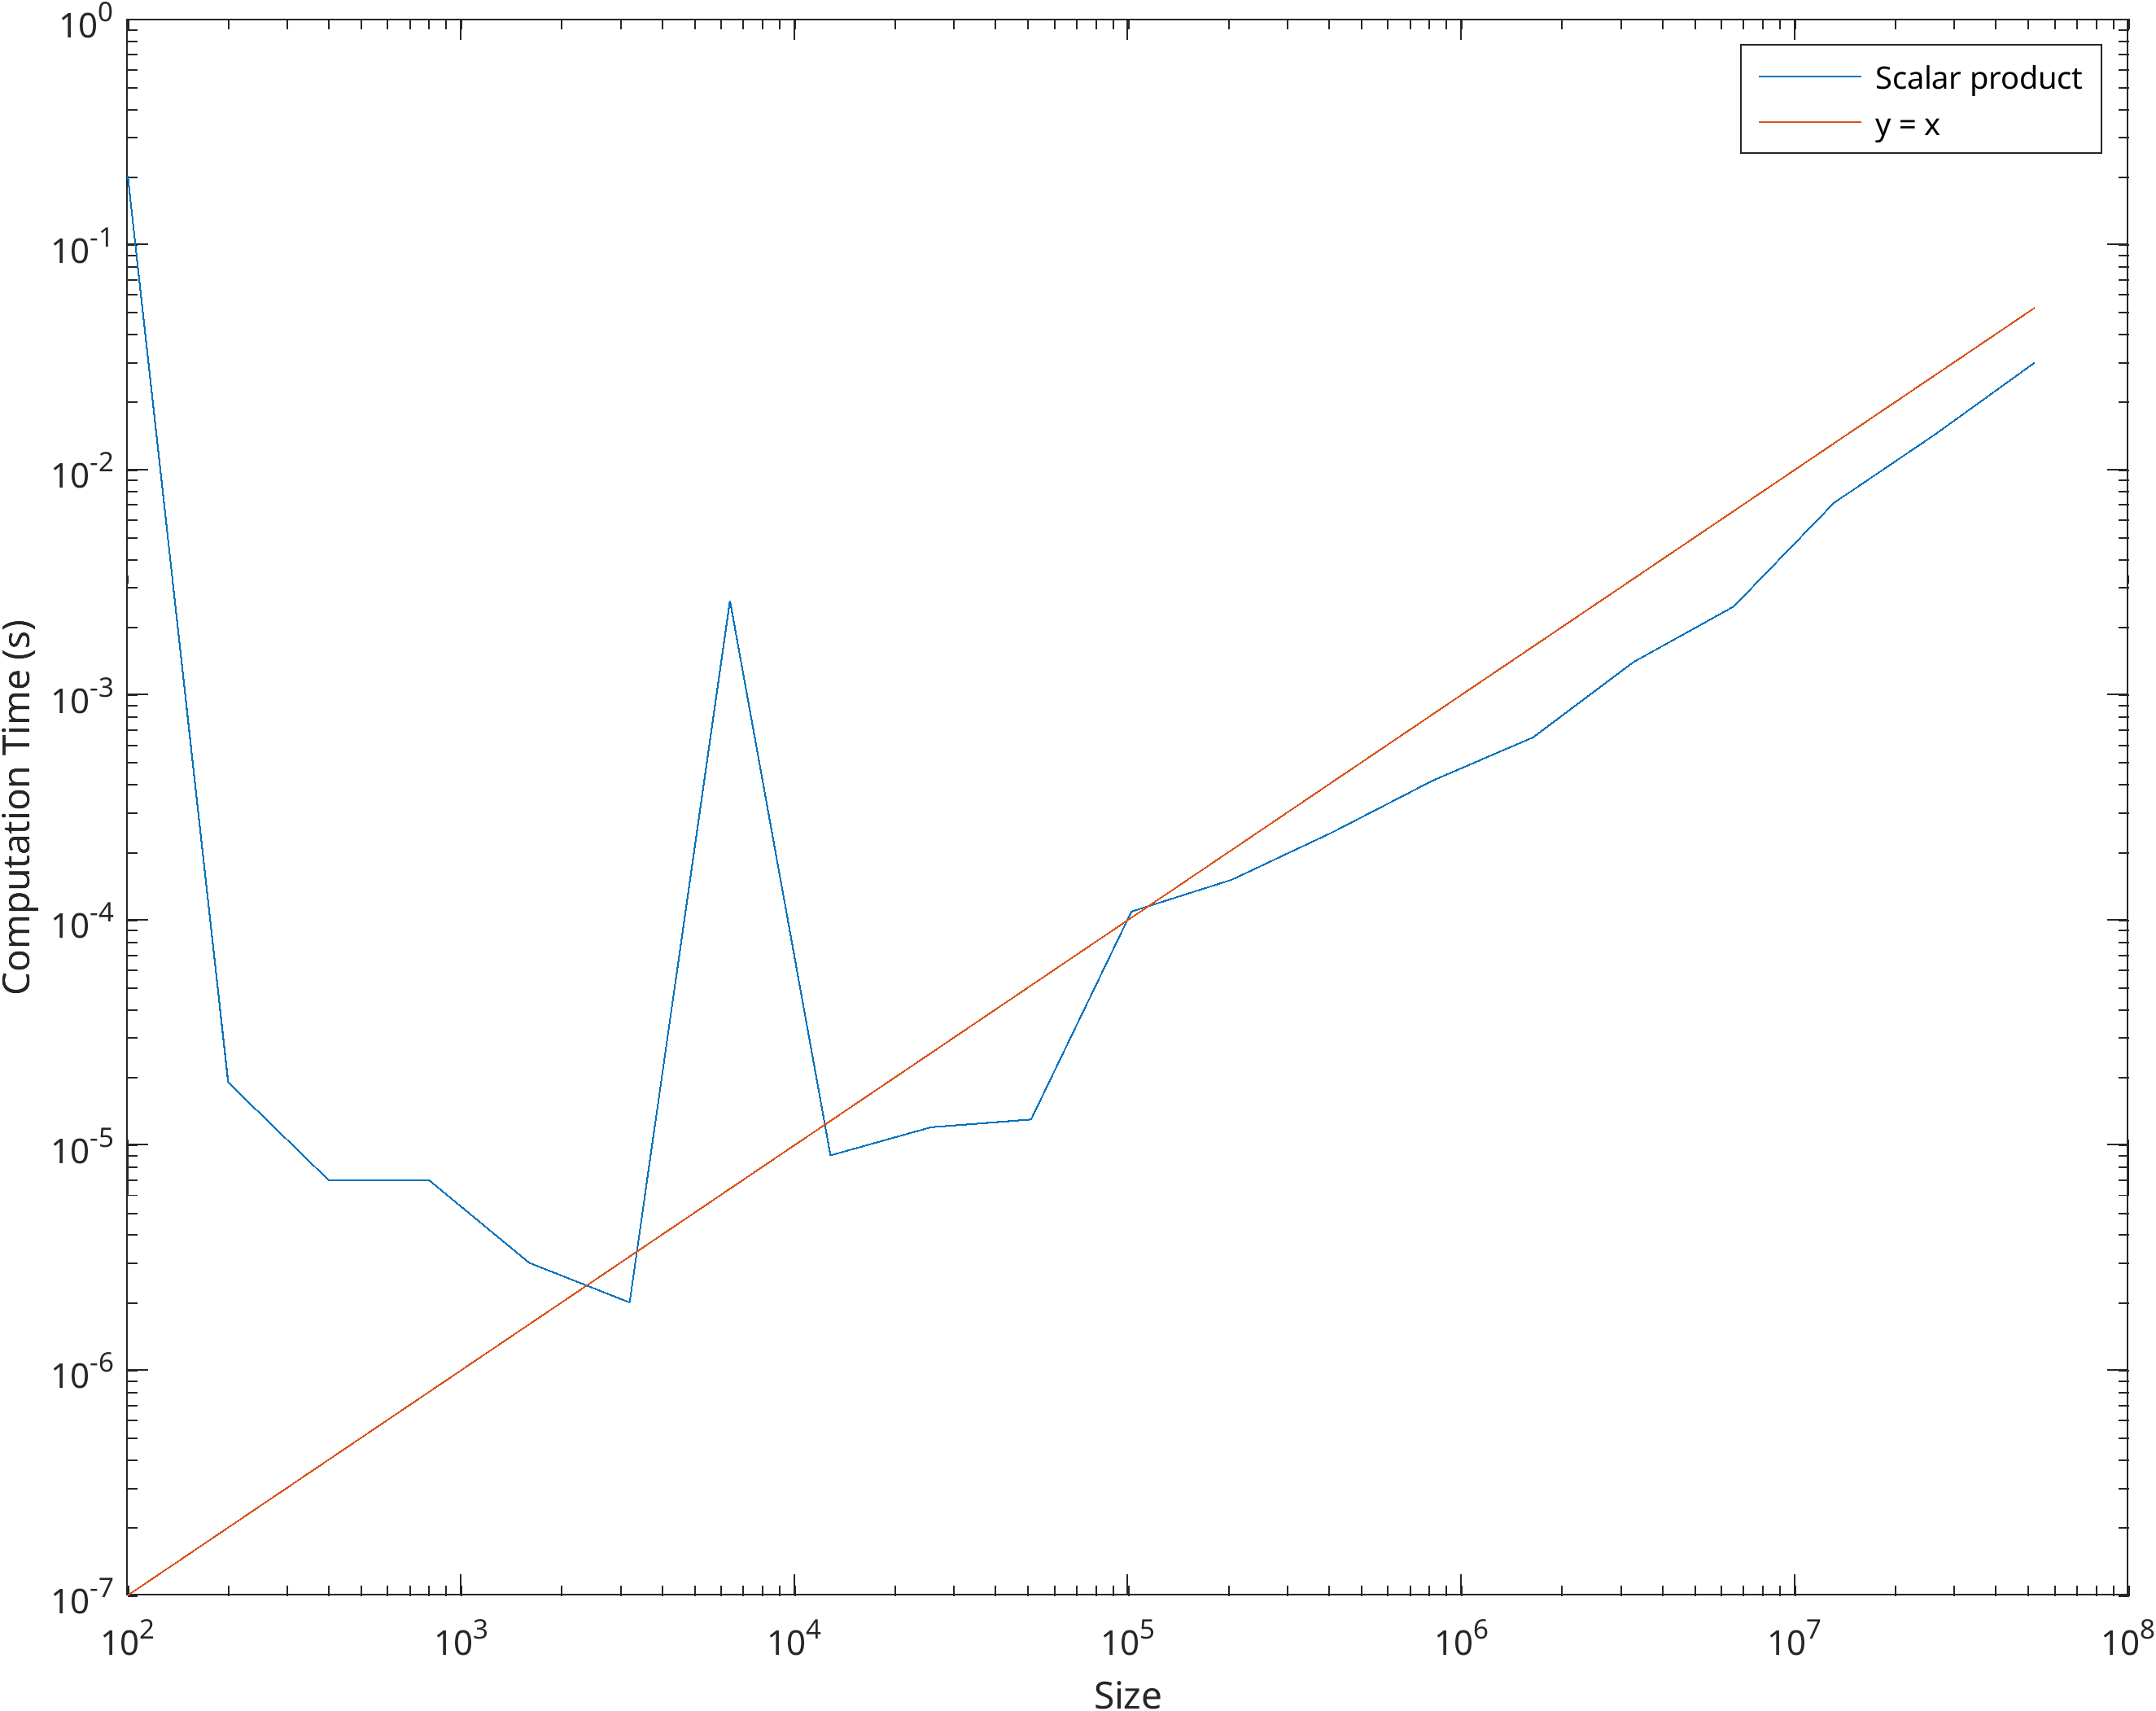
\includegraphics[scale=0.6]{../figures/scalar_perf.png}
\end{center}

Vediamo dal grafico che le prestazioni sono effettivamente vicine a quelle previste dalla complessità computazionale, se non per errori dati all'overhead di inizializzazione del timer \lstinline|tic| e \lstinline|toc| di MATLAB (lato sinistro del grafico) e della velocità generale molto elevata delle operazioni, che rende più visibile il rumore dato dallo scheduling della CPU e altri fattori di basso livello.

\item Vediamo allora l'andamento del \textbf{prodotto fra matrici}. Lo script MATLAB è praticamente identico al precedente:
\lstinputlisting{../code/matlab/time_matrix.m}
che eseguito come:
\begin{lstlisting}[language=MATLAB, style=codestyle]	
>> n = time_matrix(7);
>> hold on;
>> loglog(n, n.^3 * 10^-11);
>> hold off;
\end{lstlisting}

\begin{minipage}{\textwidth}
ci restituisce il grafico:
\begin{center}
	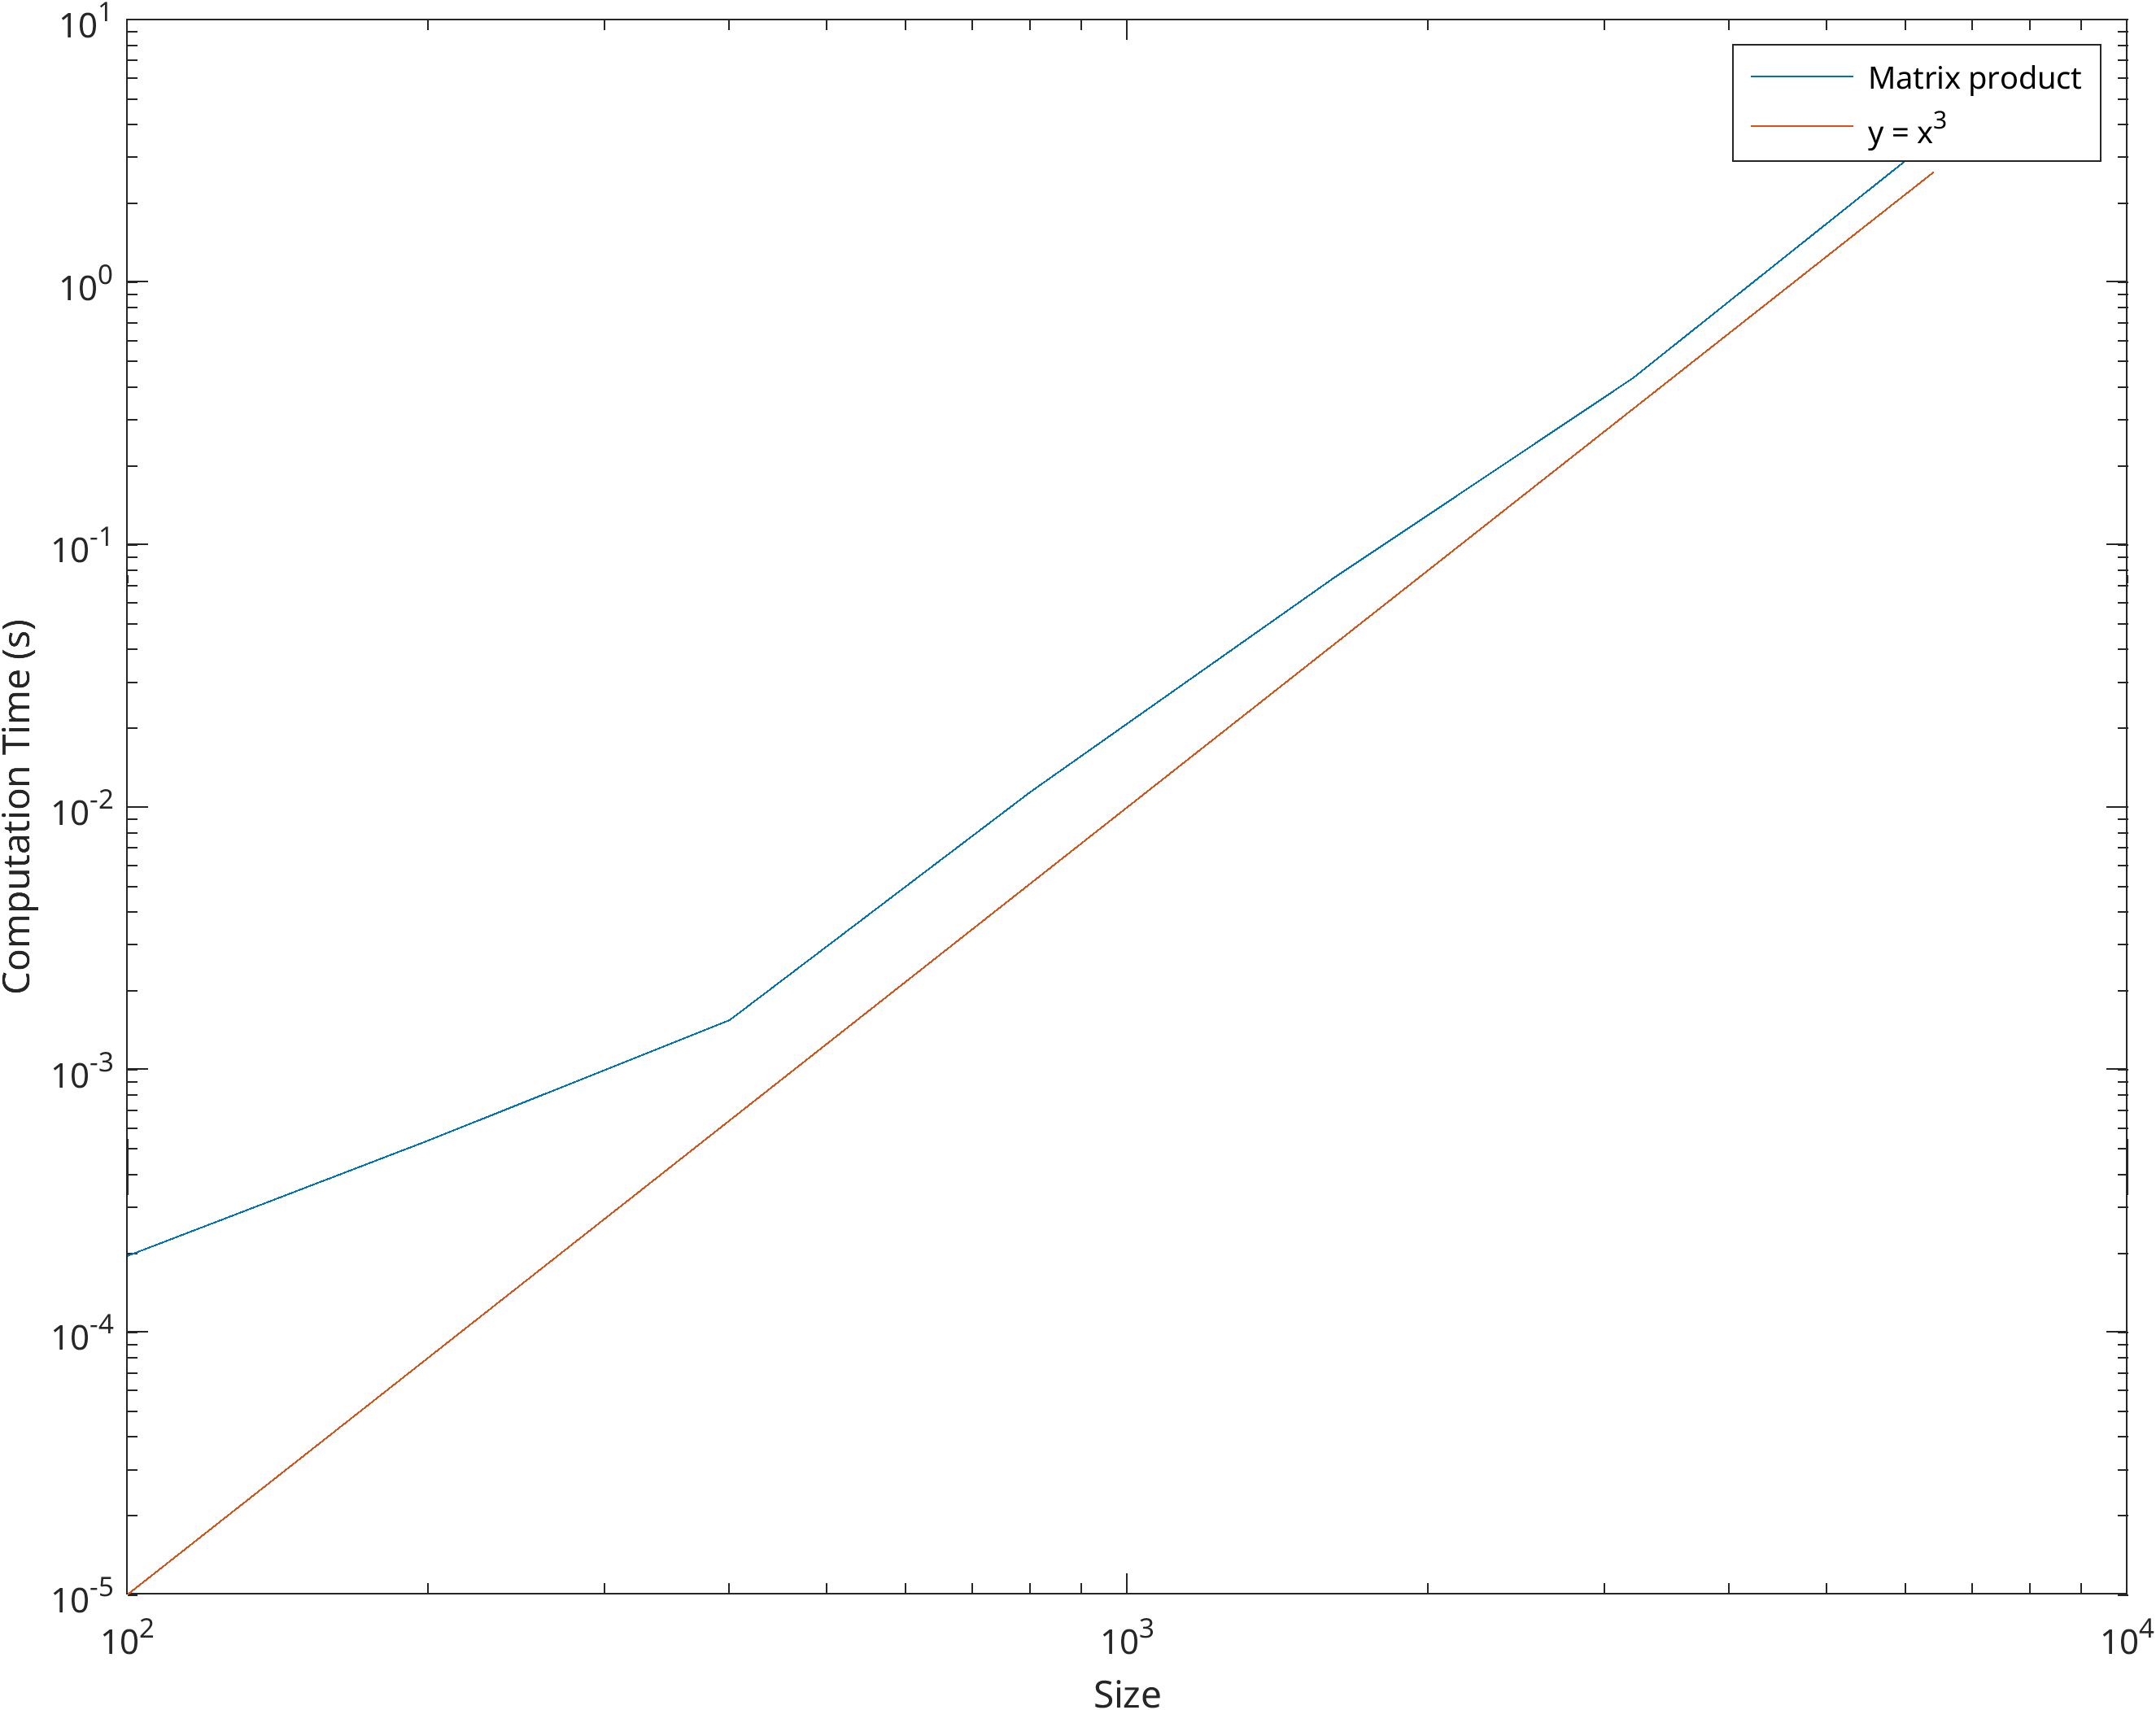
\includegraphics[scale=0.6]{../figures/matrix_perf.png}
\end{center}
che notiamo essere già più vicino del prodotto scalare (a causa del tempo di esecuzione maggiore richiesto, che "maschera" bene gli effetti a basso livello della CPU). 
\end{minipage}

\end{itemize}

\subsection{Proprietà del prodotto matriciale}
Abbiamo che in genere il prodotto fra matrici non è \textbf{commutativo}, cioè:
$$
A B \neq BA
$$
di contro, vale l'\textbf{associativa}:
$$
(A \cdot B) \cdot C = A \cdot (B\cdot C)
$$
e la \textbf{distributiva}, separatamente ai due lati:
$$
(A + B) \cdot C = A \cdot C + B \cdot C
$$
$$
C \cdot (A + B) = C \cdot A + C \cdot B 
$$

Inoltre, notiamo che quello delle matrici non è un \textit{dominio integrale}: 
$$
A \cdot B = 0 \;\not\!\!\!\implies A = 0 \vee B = 0
$$

Vediamo ad esempio come sfruttare la proprietà associativa può permetterci di ottenere algoritmi più veloci.
Supponiamo di voler calcolare:
$$
(A \cdot B) \cdot C = A \cdot (B\cdot C)
$$
con $A \in \mathbb{C}^{m \times n}$; $B \in \mathbb{C}^{n \times p}$ , $C \in \mathbb{C}^{p \times q}$.

L'uguaglianza ci darà due metodi:
\begin{itemize}
	\item $(A \cdot B) \cdot C$:
		\begin{itemize}
			\item $A \cdot B = P \in \mathbb{C}^{m \times p}, \quad O(m \cdot n \cdot p)$
			\item $P \cdot C = R \in \mathbb{C}^{m \times q}, \quad O(m \cdot p \cdot q)$
		\end{itemize}
		$\implies O(mnp + mpq) = O\left( mp (n + q) \right)$
	\item $A \cdot (B\cdot C)$:
		\begin{itemize}
			\item $B \cdot C = P \in \mathbb{C}^{n \times q}, \quad O(n \cdot p \cdot q)$
			\item $A \cdot P = R \in \mathbb{C}^{m \times q}, \quad O(m \cdot n \cdot q)$
		\end{itemize}
		$\implies O(npq + mnq) = O\left( nq (p + m) \right)$
\end{itemize}
che sono quindi uguali per $m = n = p$, ma (anche radicalmente diversi) diversi al variare di questi parametri.

In generale, quindi, se si hanno matrici con poche righe o poche colonne, è opportuno cercare di mantenere questa properietà più a lungo possibile nei risultati intermedi.

\par\smallskip

Possiamo fare considerazioni simili a quelle fatte sull'associativa con la distributiva.
Ad esempio, posta l'uguaglianza:
$$
(A + B) \cdot C = AC + BC
$$
con $A, B \in \mathbb{C}^{m \times n}$ e $C \in \mathbb{C}^{n \times p}$, abbiamo due metodi:

\begin{itemize}
	\item $(A + B) \cdot C$:
		\begin{itemize}
			\item $A + B = P \in \mathbb{C}^{m \times n}, \quad O(m\cdot n)$
			\item $P \cdot C = R \in \mathbb{C}^{m \times p}, \quad O(m \cdot n \cdot p)$
		\end{itemize}
		$
		\implies O(mn + mnp) = O\left( mn(1 + p) \right)
		$
	\item $AC + BC$:
		\begin{itemize}
			\item $A \cdot C = P_1 \in \mathbb{C}^{m \times p}, \quad O(m \cdot n \cdot p)$
			\item $B \cdot C = P_2 \in \mathbb{C}^{m \times p}, \quad O(m \cdot n \cdot p)$
		\end{itemize}
		$
		\implies O(mnp + mnp + mp) = O\left( mp(1 + 2n) \right)
		$
\end{itemize}
che sono sì asintoticamente uguali per $m = n = p$ ($O(n^3)$),  ma non esattamente uguali in quanto da un lato si ha $O(n^2 + n^3)$ e dall'altro $O(n^2 + 2 n^3)$.
Questo risulta chiaramente dal fatto che col secondo metodo decidiamo di effettuare il prodotto matriciale (che è l'operazione più costosa) non una ma 2 volte.

\par\medskip

Un altra proprietà del prodotto di matrici e che si può vedere il risultato riga per riga o colonna per colonna nei seguenti modi:
$$
A = \begin{pmatrix}
A_1 \\
... \\ 
A_m
\end{pmatrix}, \quad
B = \begin{pmatrix}
	B_1 & ... & B_p
\end{pmatrix}
$$
$$
\implies
A \cdot B = \begin{pmatrix}
	A \cdot B_1 & ... & A \cdot B_p
\end{pmatrix} = \begin{pmatrix}
A_1 B \\ ... \\ A_m B
\end{pmatrix}
$$
Questo ci dice che le colonne (le righe) di $C = A \times B$ sono combinazioni lineari delle colonne (delle righe) di $A$.

\subsection{Determinante}
Abbiamo visto la definizione di \textbf{determinante} per matrici quadrate:
\begin{definition}{Determinante}
	Si definisce la funzione:
	$$
		\mathrm{det}(A) : \mathbb{C}^{n \times n} \rightarrow \mathbb{C}
	$$
	con:
	$$
		\mathrm{det}(A) =
			\begin{cases}
				a_{11}, \quad n = 1 \\ 
				a_{11} a_{22} - a_{12} a_{21}, \quad n = 2 \\ 
				\sum_{j = 1}^n (-1)^{i + j} \mathrm{det}(A_{ij}), \quad n > 2 \quad \text{(sviluppo di Laplace)}
			\end{cases}
	$$
	determinante.
\end{definition}

Osserviamo che il calcolo del determinante attraverso lo sviluppo di Laplace ha complessità algoritmica $O(n!)$.

\subsubsection{Proprietà del determinante}
Sappiamo che $A$ invertibile $\Leftrightarrow \mathrm{det}(A)$ (cioè $A$ \textbf{singolare}).
Inoltre valgono:
$$
\mathrm{det}(A^T) = \mathrm{det}(A)
$$
$$
\mathrm{det}(A^H) = \overline{\mathrm{det}(A)}
$$

\subsection{Rango}
Vediamo poi come ci può servire il determinante delle \textbf{sottomatrici}:
\begin{definition}{Sottomatrice}
	Una sottomatrice di $A$ è una matrice ottenuta prendendo la restrizione di $A$ a un sottoinsieme di righe e di colonne, cioè data $A \in \mathbb{C}^{n \times n}$, $I, J \subseteq \{ 1, ..., n \}$ con $|I| = n_1$ e $|J| = n_2$, sarà allora:
	$$
		A(I, J) \in \mathbb{C}^{n_1 \times n_2}
	$$
	ottenuta incrociando le righe in $I$ con le colonne in $J$.
\end{definition}

Definiamo quindi i \textbf{minori}:
\begin{definition}{Minore}
	Si dice minore di ordine $k$, con $k \in \{ 1, ..., n \}$ il determinante di una sottomatrice quadrata $k \times k$.
\end{definition}

E le sottomatrici \textbf{principali} e \textbf{principali di testa}:
\begin{definition}{Sottomatrice principale}
	Una sottomatrice si dice principale se gli insiemi $I, J$ usati per estrarla sono $I = J$.
\end{definition}
\begin{definition}{Sottomatrice principale di testa}
	Una sottomatrice quadrata di ordine $k$ si dice sottomatrice principale di testa se $I = J = \{ 1, ..., k \}$.
\end{definition}
Allo stesso modo si possono definire \textbf{matrici di coda} (basterà prendere indici da $k$ ad $n$).

Possiamo quindi definire il \textbf{rango} di matrice:
\begin{definition}{Rango}
	Il rango $\mathrm{rank}(A)$ di una matrice $A$ è definito come il massimo numero di colonne (o di righe) linearmente indipendenti, ed è uguale all'ordine massimo dei minori $\neq 0$ in $A$.
\end{definition}

\subsubsection{Proprietà del rango}
Caso particolare del rango sarà chiaramente quello dove prendiamo come sottomatrice la matrice stessa: $\mathrm{det}(A) \neq 0 \Leftrightarrow \mathrm{rank}(A) = n$, e quindi gli insiemi delle colonne e delle righe di $A$ sono tutte linearmente indipendenti.

Si ha poi che:
$$
\mathrm{rank}(A) = \mathrm{dim}(\mathrm{Im}(A))
$$
dove $\mathrm{Im}(A)$ è la dimensione dell'\textbf{immagine} di $A$:
$$
\mathrm{Im}(A) = \left\{ y \in \mathbb{C}^m : y = Ax, \ x \in \mathbb{C}^n \right\}
$$

\subsubsection{Teorema di Binet-Cauchy}
Concludiamo enunciando il teorema di Binet-Cauchy sul determinante rispetto al prodotto matriciale.
\begin{theorem}{di Binet-Cauchy}
	Prese due matrici, $A \in \mathbb{C}^{n \times n}$ e $B \in \mathbb{C}^{n \times n}$, e $C = A \cdot B$ di dimensioni uguali, sarà:
	$$
	\mathrm{det}(C) = \mathrm{det}(A) \cdot \mathrm{det}(B)
	$$
Nel caso generale avremo $A \in \mathbb{C}^{n \times p}$ e $B \in \mathbb{C}^{p \times n}$, da cui:
$$
\mathrm{det}(C) =
	\begin{cases}
		0, \quad p \leq n \\
		\sum_j A_{[j]} \cdot B_{[j]}
	\end{cases}
$$
dove $A_{[j]}$ e $B_{[j]}$ sono i minori di ordine $n$ relativi ala stessa scelta di indici in $A$ e in $B$.
\end{theorem}

La dimostrazione di questo teorema si basa sullo sviluppo dei cofattori della matrice $A \cdot B$, dove si possono riarrangiare i termini per ottenere gli sviluppi dei cofattori delle matrici $A$ e $B$.

\subsection{Matrice inversa}
Diamo la definizione di \textbf{matrice inversa}:
\begin{definition}{Matrice inversa}
	Data $A \in \mathbb{C}^{n \times n}$ tale che $\mathrm{det}(A) \neq 0$, si definisce $A^{-1} \in \mathbb{C}^{n \times n}$ tale che:
	$$
	A \cdot A^{-1} = A^{-1} \cdot A = I
	$$
\end{definition}
Se si guarda ad $A$ come una funzione lineare $A : \mathbb{C}^n \rightarrow \mathbb{C}^n$, sarà che:
$$
A : x \rightarrow Ax, \quad A^{-1} : Ax \rightarrow x
$$
questo da:
$$
\left(A^{-1} \circ A\right) = A^{-1} y = A^{-1} A x = Ix = x
$$
\qed

\subsubsection{Proprietà della matrice inversa}
Vediamo alcune proprietà di $A^{-1}$:
\begin{enumerate}
	\item Ricordiamo di nuovo che $A^{-1}$ esiste se e solo se $\mathrm{det}(A) \neq 0$, cioè equivalentemente se $\mathrm{rank}(A) = n$, o $A$ ha spazi riga e colonna linearmente indipendenti;

		\item
Vediamo poi il calcolo di $\mathrm{det}(A^{-1})$: da $\mathrm{det}(I) = 1$, e:
$$
\det(A \cdot A^{-1}) = \det(A) \cdot \det(A^{-1}), \quad \text{(Binet)}
$$
$$
\implies \det(A^{-1}) = \frac{1}{\det(A)}
$$

\item Vediamo poi che:
$$
(A \cdot B)^{-1} = B^{-1} A^{-1}
$$
per matrici quadrate $A, B \in \mathbb{C}^{n \times n}$;

\item Riguardo alle trasposte e alle Hermitiane vale:
	$$
		(A^T)^{-1} = (A^{-1})^T = A^{-T}
	$$
	$$
		(A^H)^{-1} = (A^{-1})^H = A^{-H}
	$$
	e:
	$$
	(AB)^T = B^T A^T
	$$
	$$
	(AB)^H = B^H A^H
	$$
\end{enumerate}

\subsection{Matrici particolari}
Definiamo alcune matrici particolari:
\begin{definition}{Matrici particolari}
	Data $A \in \mathbb{C}^{n \times n}$, si dice di $A$ che è:
	\begin{itemize}
		\item \textbf{Hermitiana:} $A = A^H$; 
		\item \textbf{Antiermitiana:} $A = -A^H$;
		\item \textbf{Unitaria} $A^H A = A A^H = I$, $A^{-1} = A^H$;
		\item \textbf{Normale} $A^H A = A A^H$;
		\item \textbf{Simmetrica} $A = A^T$;
		\item \textbf{Antisimmetrica} $A = -A^T$;
		\item \textbf{Ortogonale} $A^TA = AA^T = I$, $A^T = A^{-1}$
	\end{itemize}
\end{definition}
dove notiamo che \textbf{simmetrica} e \textbf{antisimmetrica} significano \textit{hermitiana} e \textit{antihermitiana} in $\mathbb{R}$, e \textbf{ortogonale} significa \textit{unitaria} in $\mathbb{R}$.

Per di più vale:
$$
\{ \text{matrici simmetriche reali} \} \subseteq \{ \text{matrici hermitiane} \} \subseteq \{ \text{matrici normali} \}
$$
e:
$$\{ \text{matrici ortogonali} \} \subseteq \{ \text{matrici unitarie} \}
$$
dove notiamo che unitarie ed ortogonali hanno l'inversa "facile", nel senso che basta trasporre o trovare l'hermitiana.

\subsection{Matrici di permutazione}
Definiamo le \textbf{matrici di permutazione}:
\begin{definition}{Matrice di permutazione}
	$A \in \mathbb{R}^{n \times n}$ si dice matrice di permutazione se $A$ si ottiene dalla matrice di identità permutandone righe e colonne.
\end{definition}

\subsubsection{Proprietà delle matrici di permutazione}
Tutte le matrici di permutazione sono matrici ortogonali (questo si vede dalla loro unimodularità, o osservando che $P^T$ si ottiene dalla permutazione inversa).

Inoltre, vediamo che il prodotto di $A$ con una matrice di permutazione si limita a scambiare righe e colonne in accordo con la permutazione della matrice.
In particolare, $A \cdot P$ dà la permutazione delle colonne, mentre $P \cdot A$ dà la permutazione delle righe.

\subsection{Sistemi lineari}
Abbiamo un sistema di $m$ equazioni lineari in $n$ incognite:
\[
	\begin{cases}
		a_{11} x_1 + ... a_{1n}	x_n = b_1 \\ 
		... \\
		a_{m1} x_1 + ... a_{mn}	x_n = b_m
	\end{cases}
\]

Ci è spesso utile riscrivere sistemi di questo tipo in forma matriciale:
$$
A = \begin{pmatrix}
	a_{11} & ... & a_{1n} \\ 
	... & ... & ... \\
	a_{m1} & ... & a_{mn}
\end{pmatrix} \in \mathbb{C}^{m \times n}, \quad
x = \begin{pmatrix}
	x_1 \\ ...\\ x_n
\end{pmatrix} \in \mathbb{C}^{n}, \quad
b = \begin{pmatrix}
	b1 \\ ... \\ b_m
\end{pmatrix} \in \mathbb{C}^{m}
$$

Il problema principe sarà quello, date $A$ e $b$, di trovare $x$.

\subsubsection{Teorema di Rouché-Capelli}
Richiamiamo il teorema:
\begin{theorem}{di Rouché-Capelli}
	$Ax = b$ ammette almeno una soluzione se $\mathrm{rank}(A) = \mathrm{rank}(A | b)$, con $(A|b) \in \mathbb{C}^{m \times (n + 1)}$ la matrice ottenuta aumentando $A$ con $b$.

	Per quanto riguarda l'unicità, supposto $m \geq n$ (sistema \textit{sovradeterminato}):
	\begin{itemize}
		\item Se $\mathrm{rank}(A) = n$ allora la soluzione è unica;
		\item Se $\mathrm{rank}(A) < n$ allora ci sono $\infty$ soluzioni, e l'insieme delle soluzioni forma uno spazio vettoriale affine di dimensione $n - \mathrm{rank}(A)$;
	\end{itemize}
\end{theorem}

Nel caso il vettore $b = 0$, il sistema si dice \textbf{omogeneo}, e la soluzione nulla esiste sempre.

Abbiamo poi che:
\begin{definition}{}
	L'insieme delle soluzioni di $Ax = 0$ si chiama Kernel (nucleo) della matrice:
	$$
		\mathrm{ker}(A) = \left\{ x \in \mathbb{R}^n : Ax = 0 \right\}
	$$
\end{definition}
notiamo che il kernel è un sottospazio vettoriale di dimensione $n - \mathrm{rank}(A)$.

Osserviamo infine che nel caso $m = n$, se $\det(A) \neq 0$, cioè $\mathrm{rank}(A) = n$, la soluzione di $Ax = b$ è unica per ogni $b \in \mathbb{R}^m$ e si scrive:
$$
x = A^{-1} b
$$

Vedremo che in generale calcolare l'inversa non è conveniente rispetto ad altri metodi di approssimazione.

\subsubsection{Regola di Cramer}
Il vettore soluzione si può scrivere ache componente per componente come:
$$
x_j = \frac{\det(A_j)}{\det(A)}
$$
dove $A_j$ è la matrice ottenuta da $A$ sotituendo la colonna $j$ con $b$.

Questa via costa come calcolare $O(n)$ determinanti di matrici $n \times n$, ed è quindi poco conveniente ($O(n^3)$). 

\end{document}
